%%%%%
%%%%%


%%%%%%%%%%%%%%%%%%%%%%%%%%%%%%%%%%%%%%%%%%%%%%%%%%%%%%%%%%%%%%%%
%% Template for the papers to the case studies of Data Analytics
%%%%%%%%%%%%%%%%%%%%%%%%%%%%%%%%%%%%%%%%%%%%%%%%%%%%%%%%%%%%%%%%

\documentclass[a4paper, 12pt, titlepage, headsepline, listof = totoc, bibliography = totoc, numbers = noenddot]{scrartcl}
\usepackage[left = 3cm, right = 2cm, top = 2.2cm, bottom = 3.5cm]{geometry} % spaces on the sides of the paper
\usepackage[utf8]{inputenc}
\usepackage{graphicx}
\usepackage{amsfonts}
\usepackage{natbib}
\usepackage{scrpage2}
\usepackage{dsfont}
\usepackage{float}
\usepackage{amssymb}
\usepackage{caption}
\usepackage{subcaption}

\frenchspacing

\usepackage{bbm}
\usepackage[labelfont=bf, font=footnotesize, tableposition=top]{caption}
\DeclareCaptionType[fileext=los,placement={!ht}]{listing}
%\usepackage{mdframed}
\usepackage{boxedminipage}
%\usepackage{chngcntr}
%\def \lstWidth {0.9}

\newcommand{\eg}{e.\,g. }
\newcommand{\ie}{i.\,e. }
\newcommand{\cdf}{c.\,d.\,f. }
\newtheorem{thm}{Theorem}
\newtheorem{df}{Definition}
\newtheorem{lem}{Lemma}

%% path, where the figures are stored
\graphicspath{{./images/}}

%%%%%%%%%%%%%%%%%%%%%%%%%%%%%%%%%%%%%%%%%%%%%%%%%%%%%%%%%%%%%%%%
%% design of the head of the report pages

\clearscrheadings                   	% clears all predefined formats voreingestellte Formatierungen
\pagestyle{scrheadings}			% use this style only on the actual text
\ohead{FirstName LastName}		% writes your name on each side in the upper right corner
\automark{section}                  
\ihead{\headmark}				% automatically writtes the section name in the upper left corner
\cfoot{\pagemark}				% page number on the bottom (center)


%%%%%%%%%%%%%%%%%%%%%%%%%%%%%%%%%%%%%%%%%%%%%%%%%%%%%%%%%%%%%%%%
%% cover sheet

\title{\hrulefill \\ \vspace*{1cm} Case Studies\\\vspace*{0.5cm}
 "Data Analytics" \\ \vspace*{1cm}\hrulefill\vspace*{1.5cm}}
\subtitle{Topic\\\vspace*{1.5cm} Summer Term 2013\vspace*{1.5cm}}
\author{FirstName LastName}
%\institute{e-mail}

\usepackage{Sweave}
\begin{document}
\Sconcordance{concordance:Report.tex:D:/DA/report/DAProject/Report.Rnw:%
15 1 139 1 41 59 1 1 0 39 1 1 12 22 1 1 46 48 0 1 2 1 19 18 0 1 6 4 0 1 %
31 32 0 1 2 36 1 1 22 6 1 1 45 71 1 1 11 10 0 1 4 3 0 1 8 10 0 1 2 12 1 %
1 13 12 0 1 3 2 0 1 1 5 0 1 1 6 0 1 2 5 1 1 25 11 1 1 43 42 0 1 2 29 0 %
1 2 36 1 1 15 11 1 1 17 17 1 1 6 36 1 1 12 4 1 1 17 7 0 1 5 7 1 1 17 6 %
0 1 5 5 1 1 15 5 0 1 5 5 1 1 8 8 1 1 17 6 0 1 5 7 1 1 17 5 0 1 5 7 1 1 %
2 11 0 1 1 9 0 1 1 9 0 1 1 9 0 1 2 4 1 1 17 6 0 1 5 8 1 1 17 6 0 1 5 8 %
1 1 17 6 0 1 5 8 1 1 17 5 0 1 5 12 1 1 7 3 1 1 17 7 0 1 5 7 1 1 17 6 0 %
1 5 7 1 1 8 6 1 1 8 10 1 1 17 6 0 1 5 7 1 1 17 5 0 1 5 109 1 1 17 7 0 1 %
5 5 1 1 17 6 0 1 5 5 1 1 17 6 0 1 5 5 1 1 17 5 0 1 5 6 1 1 8 6 1 1 8 6 %
1 1 8 6 1 1 8 23 1}

\thispagestyle{empty}
\maketitle

%%%%%%%%%%%%%%%%%%%%%%%%%%%%%%%%%%%%%%%%%%%%%%%%%%%%%%%%%%%%%%%%
%% table of contents

\thispagestyle{empty}
\tableofcontents

%%%%%%%%%%%%%%%%%%%%%%%%%%%%%%%%%%%%%%%%%%%%%%%%%%%%%%%%%%%%%%%%
%% the document itself

\newpage
\setcounter{page}{1}
\section{Introduction}

\subsection{Normality as a requirement for statistical methods}

test test test

\subsection{The glass data sample}

\subsection{Aim and structure}

\newpage
\section{Preliminaries}

\subsection{Test methods for normality}\label{sec:methods}

A statistical hypothesis test which tests empirical data on conformance with a certain distribution (or a family of distributions) is called a goodness of fit test. The null hypothesis is usually the hypothesis that the tested sample has been drawn from a population which is distributed according to the given distribution. Consequently, the alternative hypothesis states that the sample was drawn from a population of any other distribution. In every test, a certain method is used to calculate a test statistic from the data. If the test statistic exceeds a critical value which is computed for the particular distribution and a certain significance level, the null hypothesis is rejected. The p-value is the lowest significance level for which the null hypothesis would still be rejected. It can be interpreted as the probability of getting a result like the present one or an even more extreme result if the null hypothesis is true.

\subsubsection{Q-Q-plot}

\subsubsection{Shapiro-Wilk test}

\subsubsection{Pearson's chi-squared test}\label{sec:chisq-theoretical}
Pearson's chi-squared goodness of fit test is used to test whether data from a sample are distributed according to an arbitrary theoretical distribution. The main idea of this test is to divide the observations $X_1, \dots, X_N$ into several pairwise disjoint classes $C_1, \dots, C_K$ and compare the empirical frequencies within these classes to the theoretical frequencies, which are expected if the data complies to the hypothetical distribution.
\begin{figure}[h!]
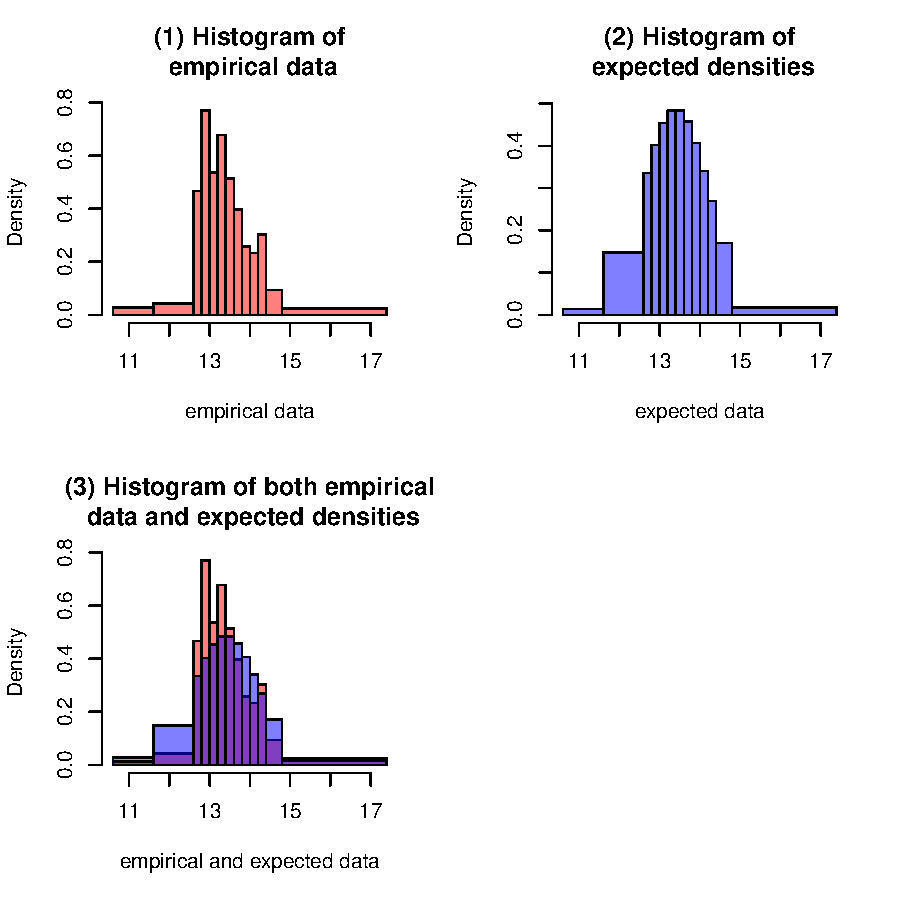
\includegraphics[width=\textwidth]{report-chisqSampleHist}
\caption{Exemplary histrograms of a data sample, expected densities for a normal distribution with parameters estimated from the sample and a combined histogram of these both histograms.}
\label{fig:chisqSampleHist}
\end{figure}
If the histograms of the sample data and the expected densities are plotted together (see figure \ref{fig:chisqSampleHist}), the area of density that is not overlapped by both histograms can be understood as a kind of indicator for the likelihood that the sample is drawn from a population which is distributed according to the hypothetical distribution: The more area is not overlapping, the less likely it is that the sample is drawn from a population with the assumed distribution. However, the test statistic of the chi-squared test is calculated differently, namely by the sum of the squared differences between observed frequencies $O_k$ and expected frequencies $E_k$ divided by the expected frequencies for each class $k$ of the overall $K$ classes. Thus, the test statistic is calculated by
\[\chi^2 = \sum_{k=1}^{K}\frac{(O_k - E_k)^2}{E_k}\]
Larger differences of observed and expected values indicate a lower compliance to the assumed distribution. However, the addends are not weighted (neither by the size of a class nor by the frequencies within a class nor by any other means). Therefore, the class bounds should be chosen equidistant or in such a way that the classes contain preferably the same number of observations or according to similar reasonable rationales. The test statistic is approximately $\chi^2$-distributed with $K-1$ degrees of freedom -- the larger the sample size, the better the approximation. A sample size that is too small can be a reason for the approximation being insufficient. Moreover, for each parameter of the hypothetical distribution which is estimated from the data sample, one degree of freedom is lost; the number of estimated parameters is denoted by $p$. The test statistic is determined under the null hypothesis that the sample is distributed according to the assumed distribution and the chi-squared test is defined as
%\[\phantom{\quad \textrm{with}\ F=\chi^2_{K-1-p}} \delta(Y) = \mathbbm{1}_{\{\chi^2\, >\, F^{-1}(1-\alpha)\}} \quad \mbox{with}\ F=\chi^2_{K-1-p}\]
\[
  \phantom{\quad\mbox{with}\ F=\chi^2_{K-1-p}}
  \delta(Y) =
   \left\{ 
    \begin{array}{cll}
%\vspace{12pt}
                 1 & \mbox{if} \ \chi^2 > F^{-1}(1-\alpha)\\
                 0 & \mbox{otherwise}
    \end{array} 
   \right.
   \quad\mbox{with}\ F=\chi^2_{K-1-p}
\]
for a given significance level $\alpha$ where $Y$ is a multinomial distributed random variable denoting the counts of observations in each class with $Y_k = |\{i : X_i \in C_k\}|$.

As a common requirement for a sufficient approximation, the minimum number of observations in each class should not fall below five. Hence, marginal or even inner classes have to be unified in some cases in order to achieve a sufficient class size. The following R-function is used here for this purpose.
\begin{Schunk}
\begin{Sinput}
 # Calculates bounds of bins (classes) of a data sample.
 # The initial bounds are given by initial_breaks,
 # k denotes the minimum class size.
 makebins = function(data, initial_breaks, k) {
   h = hist(data, breaks=initial_breaks, plot=FALSE)
   
   br = h$breaks
   changed = TRUE
   
   while(changed) {
     h = hist(data, breaks=br, plot=FALSE)
     br = h$breaks
     changed=FALSE
     
     for(i in 1:length(h$counts)) {
       if(h$counts[i] < k) {
         if(i > 1 && i < length(h$counts)) {
           if(h$counts[i-1] < h$counts[i+1]) {
             br = br[-i]
             changed = TRUE
             break
           }
           else {
             br = br[-(i+1)]
             changed = TRUE
             break
           }
         }
         # index on first class
         else if(i == 1) {
           br = br[-2]
           changed = TRUE
           break
         }
         # index on last class
         else {
           br = br[-(length(h$counts))]
           changed = TRUE
           break
         }
       }
     }
   }
   return(br)
 }
\end{Sinput}
\end{Schunk}
Further functions are needed for calculating the expected frequencies, the test statistic and the result of the test (since the mean and the standard deviation are estimated from the sample, two degrees of freedom are additionally lost):
\begin{Schunk}
\begin{Sinput}
 # Calculates the expected probabilities of a normal distribution
 # with the given parameters mean and sd
 # for the given bin (class) bounds
 probabilities.exp = function(bins, mean, sd) {
   result = rep(0, length(bins)-1)
   
   result[1] = pnorm(q=bins[2], mean=mean, sd=sd)
   
   for(i in 2:(length(bins)-1)) {
     result[i] <- pnorm(q=bins[i+1], mean=mean, sd=sd)
       - pnorm(q=bins[i], mean=mean, sd=sd)
   }
   
   result[length(bins)-1] = pnorm(q=bins[length(bins)-1],
     mean=mean, sd=sd, lower.tail=FALSE)
   
   return(result)
 }
 # Returns the chi squared test statistics
 # for the given actual and expected values.
 teststat.chi = function(actual, expected) {
   sum((actual - expected)^2 / expected)
 }
 # Performs a chi squared goodness of fit test on the given data
 # for the assumption of a normal distribution.
 # Returns true if the null hypothesis (sample drawn from a
 # normal distributed population) is rejected, false otherwise.
 # The parameters are estimated from the sample.
 # The initial bounds for the classes are given by initial_breaks,
 # min denotes the minimum class size.
 # The significance level is determined by sig.
 chisq.test.norm = function(data, initial_breaks, min, sig) {
   bins = makebins(data, initial_breaks, min)
   hist = hist(data, breaks=bins, plot=FALSE)
   expected_probabilities = probabilities.exp(bins, mean(data), sd(data))
   expected_frequencies = expected_probabilities * length(data)
   teststat = teststat.chi(hist$counts, expected_frequencies)
   
   # length(bin) - 1 classes, 2 estimated parameters (mean, sd)
   df=length(bins)-4
   critical_value = ifelse(df < 1, NA, qchisq(p=1-sig, df=df))
   
   print(teststat > critical_value)
   
   return(list(hist = hist,
               expected_probabilities = expected_probabilities,
               expected_frequencies = expected_frequencies,
               teststat = teststat,
               critical_value = critical_value,
               p_value =
                 ifelse(df < 1, NA, 1 - pchisq(q=teststat, df=df)),
               rejected = teststat > critical_value))
 }
\end{Sinput}
\end{Schunk}
A drawback of Pearson's chi-squared test is its inconsistency caused by information reduction, \ie information about the data sample is lost in the process of categorising the observations in classes. As a consequence, different class bounds can lead to different test results. Furthermore, this test is rather suited for large sample sizes.

\subsubsection{Kolmogorov-Smirnov test}\label{sec:kolm-smir}
The Kolmogorov-Smirnov (KS later on) test as all other tests is used for testing
whether a given univariate sample $x=(x_1,x_2 \dots x_n)$ with unknown distribution $\mathbb{P}$ is distributed according to a completely determined
distribution $\mathbb{P}_0$. It implies a decision making between the following
two hypotheses:
\[\begin{array}{rcl}
H_0 & : & \mathbb{P} = \mathbb{P}_0,\\
H_1 & : & \mathbb{P} \ne \mathbb{P}_0.
\end{array}\]
The decision is made according to the value of KS test
statistics and a given significance level $\alpha$.

\begin{df}
For a given univariate sample $x=(x_1, x_2, \dots, x_n)$ the function
\[F_n=\frac{1}{n}\sum_{i=1}^n \mathbbm{1}_{\{x_i\le x\}}\] is called empirical
cumulative distribution function (\cdf), where $\mathbbm{1}_{\{x_i\le x\}}$ is an
indicator function defined as follows: $\mathbbm{1}_{\{x_i\le x\}}(x)=\left\lbrace 
\begin{array}{cll}
                 1 & \mbox{if} \ x_i\le x\\
                 0 & \mbox{otherwise}.
\end{array} 
\right.$
\end{df}
The exemplary graph of such a function is depicted in the Figure
\ref{fig:empiricFunc}. 

The main idea of the KS test is the analysis of the difference between the given
cumulative distribution function (\cdf) $F$ and the empirical \cdf $F_n$. Since
both theoretical and empirical functions belong to normed space of bounded
functions $\mathbb{B}(\mathbb{R})$ (all values are between 0 and 1), this difference can be measured as
a distance $\|F_n-F\|_{\infty}=\sup_{x \in \mathbb{R}}|F_n(x)-F(x)|$. Figure
\ref{fig:empiricTeorFunc} illustrates the calculated distance between the
empirical \cdf and the theoretical normal \cdf with parameters of sample mean
and sample variance. 
%\begin{figure}[h!]
%\includegraphics[width=\textwidth]{report-empiricFunc}
%\caption{Exemplary empirical \cdf of a data sample.}
%\label{fig:empiricFunc}
%\end{figure}


%\begin{figure}[h!]
%\includegraphics[width=\textwidth]{report-empiricTeorFunc}
%\caption{Exemplary empirical \cdf of a data sample.}
%\label{fig:empiricTeorFunc}
%\end{figure}
\begin{figure}[H]
\centering
\begin{subfigure}{.5\textwidth}
  \centering
  \includegraphics[width=\linewidth]{report-empiricFunc}
  \vspace{-1cm}
  \caption{}
  \label{fig:empiricFunc}
\end{subfigure}%
\begin{subfigure}{.5\textwidth}
  \centering
  \includegraphics[width=\linewidth]{report-empiricTeorFunc}
  \vspace{-1cm}
  \caption{}
  \label{fig:empiricTeorFunc}
\end{subfigure}
\caption{Empirical \cdf for Natrium vector (a) and theoretical normal \cdf with
sample mean and sample variance (b)}
\label{fig:commonFigureKStest}
\end{figure}

The KS test statistics is defined as follows:
\[D_n = \sqrt{n}\cdot \sup_{x \in \mathbb{R}}|F_n(x)-F(x)|.\]
If value $D_i$ is considered for different $1\le i\le n$, then the sample
$\hat{D}_n=(D_1,\dots,D_n)$ is obtained that also complies with some
distribution $\mathbb{D}_n$.
It can be shown that if hypothesis $H_0$ is true, then this distribution does not depend on the \cdf $F$
and therefore can be tabulated. Moreover, Kolmogorov proved that if $n$ is large
enough then the distribution function of $\mathbb{D}_n$ can be approximated by
Kolmogorov-Smirnov distribution function
$H(t)=1-2\sum_{i=1}^{\infty}(-1)^{i-1} \exp^{-2i^2t^2}$, \ie for each positive
value $t$ the probability $P(D_n\le t)\to H(t)$ when $n \to \infty$. More
details can be found in the textbook \cite{De02}.

The KS test uses the decision rule
\[ \delta = 
\left\{
\begin{array}{rcl}
H_0&:& D_n\le c\\
H_1&:& D_n> c
\end{array}
\right.,
\]
where the critical value $c$ depends on the significance level $\alpha$ and
can be calculated from the following equations:
\[\alpha = P(\delta \ne H_0|H_0)=P(D_n>c|H_0)=1-P(D_n\le c|H_0)\approx 1-H(c).\]
As was mentioned above the last equality can be considered only when $n$ is
relatively high. Otherwise the table values for $\mathbb{D}_n$ distribution
should be used. Hence, $c\approx H^{-1}(1-\alpha)$.

Although the KS test is commonly used is has a huge drawback. Namely it
considers only completely defined theoretical \cdf. In case of normality testing
both parameters $\mu$ and $\sigma$ have to be predefined. But usually they are
a priori unknown when a sample is going to be tested. Of course it can be
managed by assigning sample mean and sample variance as unknown parameters (and
initial KS test suggests to do that) but they are not always the best choice.
Further example of Natrium distribution illustrates this proposition. 

For Natrium (Na) univariate sample of 70 observatons the sample mean
$\bar{\mu}=$13.2423 and the sample variance $\bar{\sigma}=$
0.2493 are calculated. For these values of
theoretical c.d.f. is determined (Figure \ref{fig:empiricTeorFunc}). Then
the value of KS statistics is calculated: $D_n=\sqrt{n}\cdot
\sup_x|F_n(x)-F(x)|=$2.2493.
Critical value for the significance level $\alpha=0.01$ is equal to
$c=H^{-1}(1-\alpha)$=1.6276. To
calculate this value the following $R$ functions are used:

\begin{Schunk}
\begin{Sinput}
 #Calculates KS distribution function
 H= function(t) {
 	i=1
 	sum=0
 	while(abs(f(t,i) - f(t,i+1))>0.000000000001) {
 		sum=sum+f(t,i)
 		i=i+1
 	}
 	1-2*sum
 }
 #Summand of H function
 f=function(t,i) {
 	(-1)^(i-1)*exp(-2*i^2*t^2)
 }
 #Returns value c such that H(c)=a 
 Inverse = function(H,a) {
 	newFunction = function(t) {
 		H(t)-a
 	}
 	#Returns the root of the equation H(x)-a=0
 	uniroot(newFunction,c(0.2,4),tol=0.001)$root
 }
\end{Sinput}
\end{Schunk}
Since $D_n>c$ the null hypothesis is rejected by KS test. But that does not mean
that the sample is not normal distributed. That means only that it is not normal
distributed with sample mean and sample variance as parameters of that
distribution. 

In order to manage that issue KS test is improved by solving the following
optimization problem \[KS(\mu,\sigma)=\sup_{x \in
\mathbb{R}}|F_n(x)-F(x,\mu,\sigma)|\to \min.\]
When the new values $\hat{\mu}$ and $\hat{\sigma}$ that minimize the value
$KS(\mu,\sigma)$ are found the general KS test is performed with respect to
these values of parameters. For solving this optimization problem the following
$R$ code is used:

\begin{Schunk}
\begin{Sinput}
 KS= function(param) {
 	#discretization of a line segment
 	seq = seq(from = min(dat)-0.2, to = max(dat)+0.2, length.out=1000)
 	#values of empirical c.d.f.
 	empdat = sapply(seq, function(x) {empiric(x,dat)})
 	#values of theoretical c.d.f.
 	theordat = pnorm(seq,param[1],abs(param[2]))
 	#difference between the values
 	dif=theordat-empdat
 	absdiff=abs(dif)
 	max(absdiff)
 }
 #optim is a predifined R function in stats package
 #defalut method of optimization is Nelder and Mead (1965)
 KSoptim = optim(c(mean,Cov),KS)
 KSoptim$par
\end{Sinput}
\begin{Soutput}
[1] 13.1769501  0.4682486
\end{Soutput}
\begin{Sinput}
 KSoptim$value
\end{Sinput}
\begin{Soutput}
[1] 0.07870673
\end{Soutput}
\end{Schunk}
These new parameters
$\hat{\mu}=$13.1770 and
$\hat{\sigma}=$0.4682 are taken as
parameters of a new theoretical normal \cdf and a new distance is calculated
(Figure \ref{fig:improvedKS}). 
\begin{figure}[H]
\includegraphics[width=\textwidth]{report-improvedKS}
\caption{Normal \cdf with optimized parameters in comparison to the old \cdf
with sample mean and sample variance.}
\label{fig:improvedKS}
\end{figure}

The new value of KS statistics is $D_n=\sqrt{n}\sup_{x \in
\mathbb{R}}|F_n(x)-F(x,\hat{\mu},\hat{\sigma})|=$0.6585
that is smaller than the critical value $c=$1.6276. Therefore the null
hypothesis $H_0$ is accepted by KS-test. For all further samples the improved KS
test is used. It was implemented in $R$ and has the following code.

\begin{Schunk}
\begin{Sinput}
 # Performs a Kolmogorov-Smirnov goodness of fit test on the given data
 # for the assumption of a normal distribution.
 # Returns true if the null hypothesis (sample drawn from a
 # normal distributed population) is rejected, false otherwise.
 # The parameters are optimized.
 # The significance level is determined by sig.
 KSimpr.test.norm = function(data, sig) {
 	critical_value = Inverse(H,1-sig)
 	#Sample mean and sample variance calculation
 	mu = mean(data)
 	sigma = var(data)
 	#KS function that has to be minimized.
 	KS= function(param) {
 		#discretization of a line segment
 		seq = seq(from = min(data)-0.2, 
 				to = max(data)+0.2, length.out=1000)
 		#values of empirical c.d.f.
 		empdat = sapply(seq, function(x) {empiric(x,data)})
 		#values of theoretical c.d.f.
 		theordat = pnorm(seq,param[1],abs(param[2]))
 		#difference between the values
 		dif=theordat-empdat
 		absdiff=abs(dif)
 		max(absdiff)
 		}	
 	#optim is a predifined R function in stats package
 	#defalut method of optimization is Nelder and Mead (1965)
 	KSoptim = optim(c(mu,sigma),KS)
 	teststat = sqrt(length(data))*KSoptim$value
 	p_value = 1-H(teststat)
 	
 	print(teststat > critical_value)
 	
 	return(list( mean = mu,
 				var = abs(sigma),
 				mu_opt = KSoptim$par[1],
 				sigma_opt = abs(KSoptim$par[2]),
 				teststat = teststat,
 				critical_value = critical_value,
 				p_value = p_value,
 				rejected = teststat > critical_value))
 }
 KSimpr.test.norm(dat,0.01)
\end{Sinput}
\begin{Soutput}
[1] FALSE
$mean
[1] 13.24229

$var
[1] 0.2493019

$mu_opt
[1] 13.17695

$sigma_opt
[1] 0.4682486

$teststat
[1] 0.6585078

$critical_value
[1] 1.627616

$p_value
[1] 0.7787185

$rejected
[1] FALSE
\end{Soutput}
\end{Schunk}

The problem of approximation with $H$ function remains in the improved KS test
as well. Therefore this approximation is only applicable when 
the sample size is relatively high. Otherwise the tabular values for
$\mathbb{D}_n$ distribution should be used. 



\subsection{Box-Cox-transformation}

If data is not normally distributed, it can still be transformed to fit to a normal distribtion in some cases. One possibility is the Box-Cox-transformation. It is a family of parameterised power tranformations:
\[
  \phantom{\quad\mbox{for}\ x > 0}
   x^{(\lambda)} =
   \left\{ 
    \begin{array}{cl}
%\vspace{12pt}
                 \frac{x^\lambda - 1}{\lambda} & \lambda \neq 0\\
                 \ln(x) & \lambda = 0
    \end{array}
   \right.
   \quad\mbox{for}\ x > 0
\]
The optimal parameter for specific observations $x_1, \dots, x_n$ can be determined by a maximum-likelihood estimation, maximising the log likelihood
\[
\begin{array}{l}
\vspace{12pt}
   l(\lambda) = - \frac{n}{2}\ln\left[\frac{1}{n}\sum_{j=1}^{n}(x_j^{(\lambda)} - \overline{x^{(\lambda)}})^2\right] + (\lambda - 1) \sum_{j=1}^{n}\ln(x_j)\\
   \mbox{with}\ \overline{x^{(\lambda)}} = \frac{1}{n} \sum_{j=1}^{n}x_j^{(\lambda)}
\end{array}
\]
However, a Box-Cox-transformation does not ensure that the data is normally distributed thereafter. One reason that a sample cannot be properly transformed could be that it is not unimodal. Histograms and QQ-plots of a sample from a unimodal distribution are depicted in figure \ref{fig:transformationUnimodal}. Data that is generated from a Weibull distribution can be transformed to approximately normally distributed values quite well as can be recognised by the histogram and the QQ-plot. In contrast, it is not possible to properly transform a sample that is combined from two different distributions (here with different scale parameters of the Weibull distribution) as shown in figure \ref{fig:transformationBimodal}. By the combination of two samples with different mean values a bimodal sample emerges preventing the underlying data to be transformed to a unimodal sample (namely a normally distributed sample) by a simple function. Furthermore, noisy data is not suited for Box-Cox-transformation either because the Box-Cox-function is applied on the whole sample (and not only the "noisy parts").
\newpage
\phantom{.}
\vfill

\begin{figure}[h!]
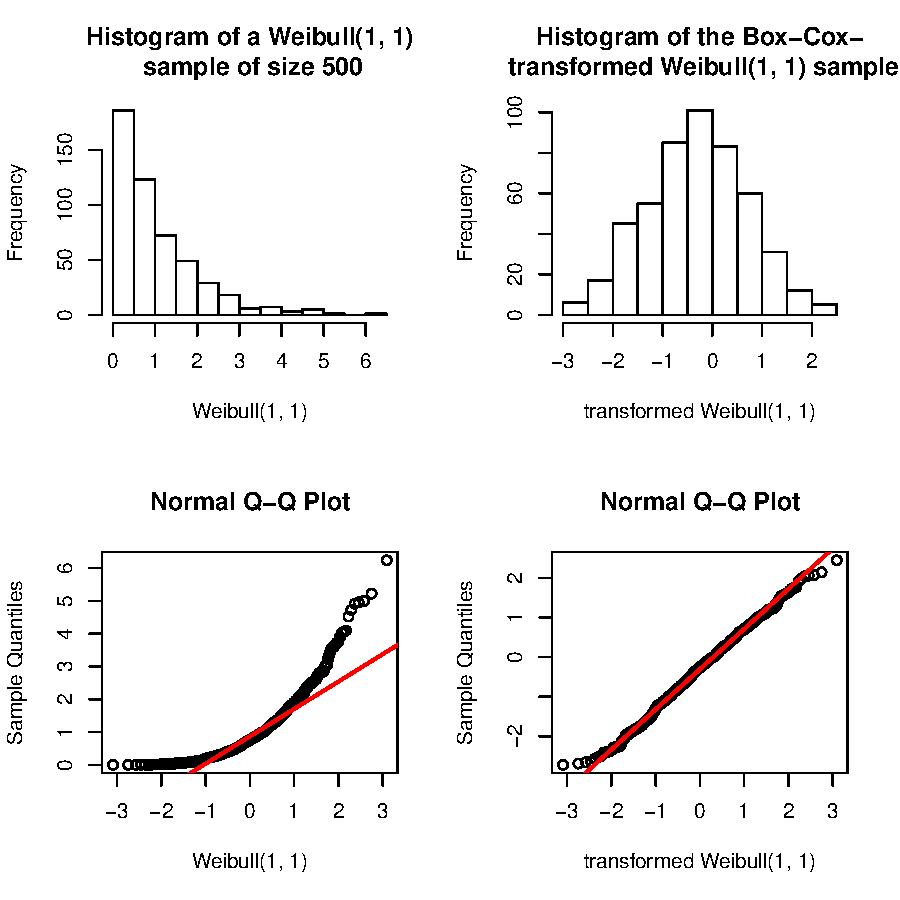
\includegraphics[width=\textwidth]{report-transformationUnimodal}
\caption{Histograms and QQ-plots of a Weibull(1, 1) simulated sample of size 500 and of the Box-Cox-transformed data}
\label{fig:transformationUnimodal}
\end{figure}

\vfill

\newpage
\phantom{.}
\vfill

\begin{figure}[h!]
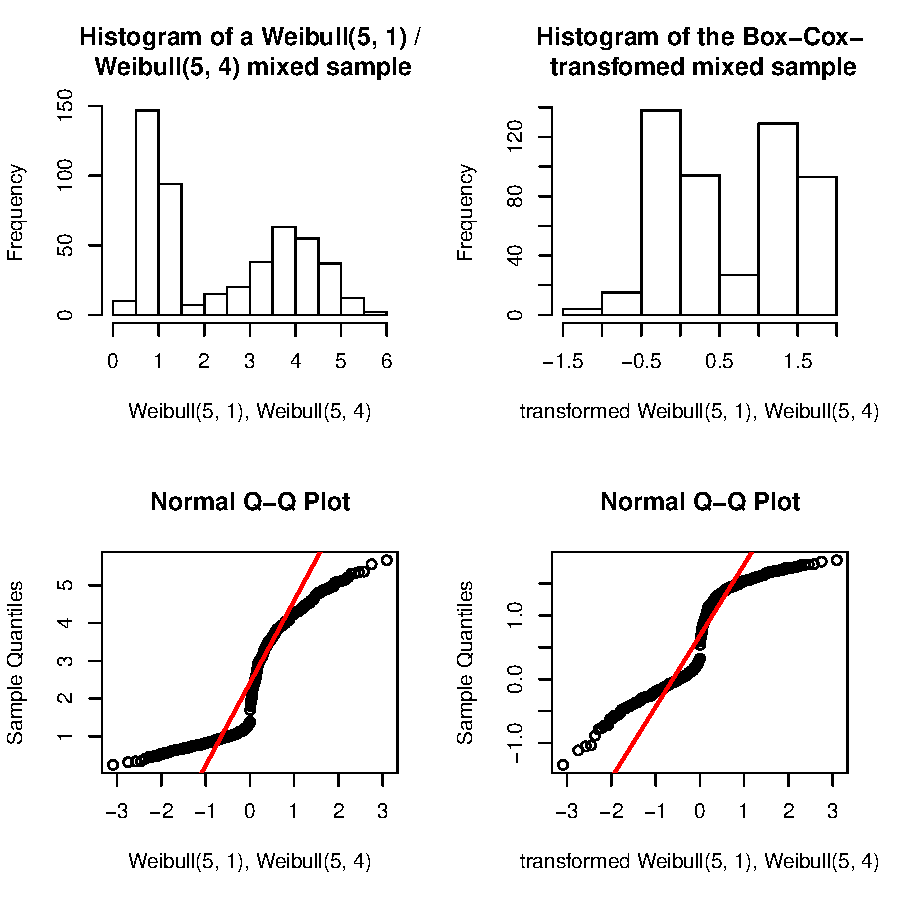
\includegraphics[width=\textwidth]{report-transformationBimodal}
\caption{Histograms and QQ-plots of a mixed sample composed of a Weibull(5, 1) simulated sample and a Weibull(5, 4) simulated sample (each of size 250) and of the Box-Cox-transformed data}
\label{fig:transformationBimodal}
\end{figure}

\vfill

\newpage
\subsection{Plot of a multivariate normal distribution}

Contour lines of the plot of a multivariate normal distribution
\[Pr(x) = |2\pi\Sigma|^{-1/2} \,\mbox{exp}\left\{-\frac{1}{2}(x-\mu)' \Sigma^{-1}(x-\mu)\right\}\]
with mean vector $\mu$ and covariance matrix $\Sigma > 0$ are shaped elliptically. Those ellipsoids are centered at $\mu : \left\{x:(x-\mu)'\Sigma^{-1}(x-\mu) = c^2\right\}$ with some constant $c$.

A first approach to check a sample of several variables on multivariate normal distribution is to examine the plot on the appearance of elliptical contour lines.

\begin{figure}[h!]
\centering
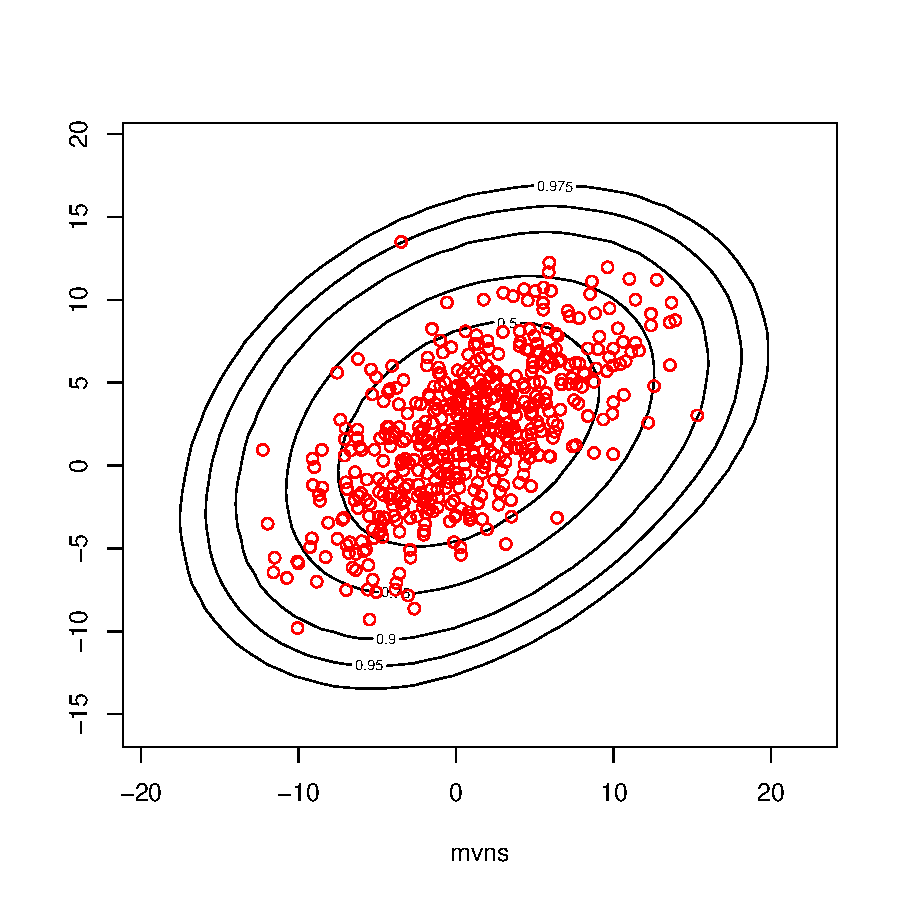
\includegraphics[width=0.8\textwidth]{report-plotMVNSim}
\caption{cap}
\label{fig:plotMVNSim}
\end{figure}



\newpage
\section{Testing the data sample for normality}

\subsection{Testing original data}

The test methods for normality that were introduced in section \ref{sec:methods} are now applied on the glass data set. For each method, the whole sample is tested first. Since it can be assumed that the different glass types are distinct in terms of the underlying distribution of variable values, the tests are conducted on the individual types as well (where applicable). It appears reasonable to skip particular variables whose values predominantly consist of zeros (more than 50\,\% of the observations, see table \ref{tab:zeros}) because this indicates that those variables are not normally distributed anyway (moreover, this can lead to complications for some methods).

\begin{table}[h!]
\centering
\begin{tabular}{|cl|}
\hline
type & skipped variables\\
\hline
1 & Ba\\
2 & Ba\\
3 & Ba, Fe\\
5 & Ba, Fe\\
6 & K, Ba, Fe\\
7 & Mg\\
\hline
\end{tabular}
\caption{Skipped variables for the particular glass types due to too many zero values}
\label{tab:zeros}
\end{table}

\subsubsection{Q-Q-plot}

\subsubsection{Shapiro-Wilk test}

\subsubsection{Pearson's chi-squared test}

As mentioned in section \ref{sec:chisq-theoretical}, Pearson's chi-squared test is not suited for rather small sample sizes because of the approximation via the chi-squared distribution. Concerning the given data, the samples of type 3 glass (17 observations), type 5 glass (13 observations) and type 6 glass (9 observations) are not large enough to ensure a viable test result. Hence, the data belonging to those types will not be considered for separate tests. However, it will remain in the overall data sample of all types. The minimum size of observations in each class is set to five and the number of initial classes (\ie number of classes before unifying) will be ten. The first tests are conducted on the whole data set for each variable. The results are shown in table \ref{tab:chi-full}. For two variables, it is not possible to determine a test result with the given parameters: The observations of the variables Potassium (K) and Barium (Ba) are divided only into three classes respectively after the unification of classes in order to fulfill the requirement of minimum class size. Since one degree of freedom is subtracted always and two degrees of freedom are subtracted for the estimation of the mean value and the standard deviation, zero degrees of freedom remain and so the critical value cannot be calculated. For each of the other variables, the hypothesis of normality is clearly rejected for the given significance level.

\begin{table}[h!]
\centering
\begin{tabular}{|cccccc|} \hline variable & test statistic & sig. level & critical value & p-value & rejected\\ \hline RI & 64.95 & 0.01 & 13.28 & 2.64011035255862e-13 & yes\\ 
Na & 36.99 & 0.01 & 13.28 & 1.80797974702607e-07 & yes\\ 
Mg & 158.3 & 0.01 & 11.34 & < 1.0e-15 & yes\\ 
Al & 27.2 & 0.01 & 9.21 & 1.24084046404516e-06 & yes\\ 
Si & 38.85 & 0.01 & 13.28 & 7.4876188027595e-08 & yes\\ 
K & 95.97 & 0.01 & NA & NA & NA\\ 
Ca & 131.13 & 0.01 & 13.28 & < 1.0e-15 & yes\\ 
Ba & 31.37 & 0.01 & NA & NA & NA\\ 
Fe & 70.96 & 0.01 & 13.28 & 1.4210854715202e-14 & yes\\ \hline \end{tabular}\caption{Test results of the chi-squared test on the whole data sample with ten initial classes}
\label{tab:chi-full}
\end{table}

The results for type 1 glass (table \ref{tab:chi-type1}) are slightly different; in this case, the results can be determined for each variable (except for Barium (Ba), which has been dropped beforehand) and the hypothesis of normality is rejected for each variable but Natrium (Na). The p-value for Natrium is comparably high amounting to approximately 0.52. It is well recognisable that the observed class frequencies for Natrium fluctuate around the expected class frequencies under the hypothesis of a normal distribution with the according parameters (table \ref{tab:testresChisqFreqNaType1}). The good compliance of empirical and hypothetical data for this variable is illustrated in figure \ref{fig:chisqType1Na}. In general, the p-values for this part of the sample are higher than those for the whole sample.

\begin{table}[h!]
\centering
\begin{tabular}{|cccccc|} \hline variable & test statistic & sig. level & critical value & p-value & rejected\\ \hline RI & 28.01 & 0.01 & 9.21 & 8.26265138420545e-07 & yes\\ 
Na & 3.25 & 0.01 & 13.28 & 0.51688441877949 & no\\ 
Mg & 18.81 & 0.01 & 6.63 & 1.44068580684165e-05 & yes\\ 
Al & 23.55 & 0.01 & 11.34 & 3.10284613768141e-05 & yes\\ 
Si & 23.68 & 0.01 & 13.28 & 9.26014020323773e-05 & yes\\ 
K & 114.86 & 0.01 & 11.34 & < 1.0e-15 & yes\\ 
Ca & 22.58 & 0.01 & 15.09 & 0.000405198755082603 & yes\\ 
Fe & 18.65 & 0.01 & 9.21 & 8.91413549507503e-05 & yes\\ \hline \end{tabular}\caption{Test results of the chi-squared test on type 1 glass with ten initial classes}
\label{tab:chi-type1}
\end{table}

\begin{table}[h!]
\centering
\begin{tabular}{|c|cc|} \hline class & \multicolumn{2}{c|}{frequencies}\\ (interval) & observed & expected\\ \hline ]12.4, 12.8] & 15 & 13.15\\ 
]12.8, 13] & 12 & 8.81\\ 
]13, 13.2] & 9 & 10.68\\ 
]13.2, 13.4] & 11 & 11.04\\ 
]13.4, 13.6] & 8 & 9.74\\ 
]13.6, 14] & 9 & 12.06\\ 
]14, 14.8] & 6 & 4.52\\ \hline \end{tabular}\caption{Observed end expected frequencies of items in the classes for the variable Natrium of type 1 glass}
\label{tab:testresChisqFreqNaType1}
\end{table}

\begin{figure}[h!]
\centering
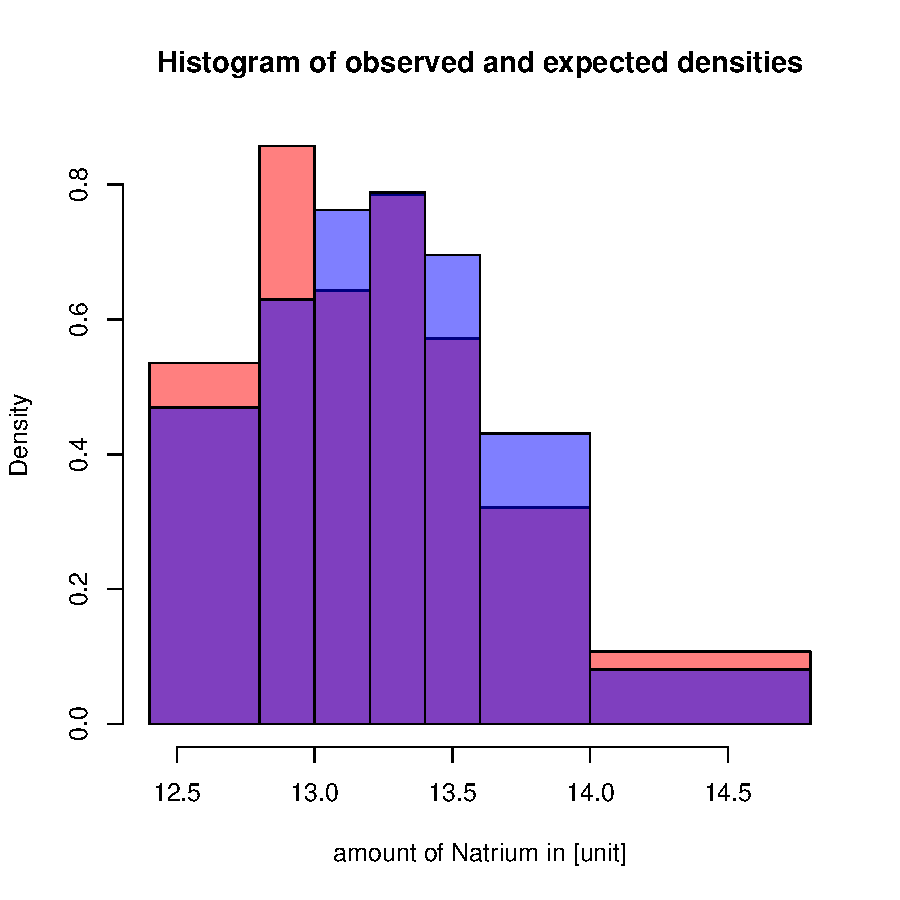
\includegraphics[width=0.8\textwidth]{report-chisqType1Na}
\caption{Histogram of observed densities (red) and expected densities (blue) within the classes for the variable Natrium of type 1 glass}
\label{fig:chisqType1Na}
\end{figure}

The test results for observations of type 2 glass are summarised in table \ref{tab:chi-type2}. The null hypothesis is rejected for all variables except for Aluminium (Al) and Silicon (Si). The p-values for these variables are however rather small (approximately 0.02 and 0.04).

\begin{table}[h]
\centering
\begin{tabular}{|cccccc|} \hline variable & test statistic & sig. level & critical value & p-value & rejected\\ \hline RI & 27.92 & 0.01 & 9.21 & 8.6430973300633e-07 & yes\\ 
Na & 8.2 & 0.01 & 6.63 & 0.00418393039163056 & yes\\ 
Mg & 66.57 & 0.01 & 6.63 & < 1.0e-15 & yes\\ 
Al & 9.41 & 0.01 & 11.34 & 0.024332262426528 & no\\ 
Si & 6.24 & 0.01 & 9.21 & 0.0441247638253744 & no\\ 
K & 41.06 & 0.01 & 6.63 & 1.47495904379014e-10 & yes\\ 
Ca & 71.68 & 0.01 & 9.21 & < 1.0e-15 & yes\\ 
Fe & 16.75 & 0.01 & 11.34 & 0.000794876178432768 & yes\\ \hline \end{tabular}\caption{Test results of the chi-squared test on type 2 glass with ten initial classes}
\label{tab:chi-type2}
\end{table}

For the observations of type 7 glass, test results (table \ref{tab:chi-type7}) are only available for the variable Aluminium (Al). Due to the small sample size of 29 observations, most of the initial classes are joined so that no degree of freedom remains for the chi-squared distribution function. The hypothesis of normality is not rejected for the data of Aluminium.

\begin{table}[h!]
\centering
\begin{tabular}{|cccccc|} \hline variable & test statistic & sig. level & critical value & p-value & rejected\\ \hline RI & 19.93 & 0.01 & NA & NA & NA\\ 
Na & 1.4 & 0.01 & NA & NA & NA\\ 
Al & 3.42 & 0.01 & 6.63 & 0.0644860281274806 & no\\ 
Si & 4.84 & 0.01 & NA & NA & NA\\ 
K & 13.14 & 0.01 & NA & NA & NA\\ 
Ca & 11.93 & 0.01 & NA & NA & NA\\ 
Ba & 0.2 & 0.01 & NA & NA & NA\\ \hline \end{tabular}\caption{Test results of the chi-squared test on type 7 glass with ten initial classes}
\label{tab:chi-type7}
\end{table}

As mentioned in section \ref{sec:chisq-theoretical}, Pearson's chi-squared test is inconsistent when the number or bounds of classes are changed. This inconsistency can also be observed with the present data set. The test have also been conducted with 30 initial classes each (see tables \ref{tab:chi-full-30} to \ref{tab:chi-type7-30} in the appendix) with partly different results. Whereas with ten initial classes, there are not enough classes left for most of the variables of type 7 glass to be tested, the data is divided in a sufficient number of classes when using 30 initial classes. Above all, the null hypothesis is not rejected for Aluminium (Al) of type 2 glass with ten initial classes but it is rejected with 30 initial classes while the opposite is true for Natrium (Na). In general, the p-values can alternate much with different classes; so the rather high p-value for Natrium of type 1 glass ($\sim$ 0.52) with ten initial classes decreases to approximately 0.02 with 30 initial classes. On the contrary, the p-value for Aluminium of type 7 glass ($\sim$ 0.06) increases to approximately 0.19. These different impacts on the test results are due to two opposing effects: First, with more classes there are more degrees of freedom for the chi-squared distribution and thus the critical value increases. Second, the test statistic tends to increase as well because the observations have to fit to smaller classes more precisely; or in other words, observations may be distorted (relatively to the hypothetical expectations) within a large class so that differences between empirical and hypothetical data do not raise the test statistic as much as the same observations would if they were divided into smaller classes (making the distortion "measurable").

\subsubsection{Kolmogorov-Smirnov test}

The first tests are conducted on the whole data set for each variable. 
The results are shown in table \ref{tab:KS-full}.

\begin{table}[h!]
\centering
\begin{tabular}{|cccccc|} \hline variable & test statistic & sig. level & critical value & p-value & rejected\\ \hline RI & 1.34 & 0.01 & 1.63 & 0.0561963016778131 & no\\ 
Na & 0.87 & 0.01 & 1.63 & 0.43825271603342 & no\\ 
Mg & 2.94 & 0.01 & 1.63 & 6.18457917100912e-08 & yes\\ 
Al & 0.84 & 0.01 & 1.63 & 0.474757887353829 & no\\ 
Si & 0.96 & 0.01 & 1.63 & 0.314710019077325 & no\\ 
K & 2.14 & 0.01 & 1.63 & 0.000212776619708754 & yes\\ 
Ca & 1.33 & 0.01 & 1.63 & 0.057710602872685 & no\\ 
Ba & 2.6 & 0.01 & 1.63 & 2.75476085742632e-06 & yes\\ 
Fe & 4.68 & 0.01 & 1.63 & < 1.0e-15 & yes\\ \hline \end{tabular}\caption{Test results of the improved KS test on the whole data sample}
\label{tab:KS-full}
\end{table}

Then tests are conducted on type 1 glass for each variable.
The results are shown in table \ref{tab:KS-type1}.

\begin{table}[h!]
\centering
\begin{tabular}{|cccccc|} \hline variable & test statistic & sig. level & critical value & p-value & rejected\\ \hline RI & 1.31 & 0.01 & 1.63 & 0.0630043926883292 & no\\ 
Na & 0.66 & 0.01 & 1.63 & 0.77871853343362 & no\\ 
Mg & 0.49 & 0.01 & 1.63 & 0.967729719418776 & no\\ 
Al & 0.92 & 0.01 & 1.63 & 0.366854549713195 & no\\ 
Si & 1.06 & 0.01 & 1.63 & 0.208027646546284 & no\\ 
K & 1.73 & 0.01 & 1.63 & 0.00491847745617136 & yes\\ 
Ca & 0.84 & 0.01 & 1.63 & 0.48064266616439 & no\\ 
Fe & 2.65 & 0.01 & 1.63 & 1.63244296669252e-06 & yes\\ \hline \end{tabular}\caption{Test results of the improved KS test on type 1 glass}
\label{tab:KS-type1}
\end{table}

After that the tests are conducted on type 2 glass for each variable.
The results are shown in table \ref{tab:KS-type2}.

\begin{table}[h!]
\centering
\begin{tabular}{|cccccc|} \hline variable & test statistic & sig. level & critical value & p-value & rejected\\ \hline RI & 1.08 & 0.01 & 1.63 & 0.190264315474967 & no\\ 
Na & 0.49 & 0.01 & 1.63 & 0.969807662718898 & no\\ 
Mg & 1.37 & 0.01 & 1.63 & 0.0477938096655182 & no\\ 
Al & 0.64 & 0.01 & 1.63 & 0.807950624660872 & no\\ 
Si & 0.55 & 0.01 & 1.63 & 0.918823986509849 & no\\ 
K & 1.18 & 0.01 & 1.63 & 0.125440771961193 & no\\ 
Ca & 1.43 & 0.01 & 1.63 & 0.0327944325987 & no\\ 
Fe & 2.5 & 0.01 & 1.63 & 7.20083142169425e-06 & yes\\ \hline \end{tabular}\caption{Test results of the improved KS test on type 2 glass}
\label{tab:KS-type2}
\end{table}

After that the tests are conducted on type 7 glass for each variable.
The results are shown in table \ref{tab:KS-type7}.

\begin{table}[h!]
\centering
\begin{tabular}{|cccccc|} \hline variable & test statistic & sig. level & critical value & p-value & rejected\\ \hline RI & 0.67 & 0.01 & 1.63 & 0.767837508224946 & no\\ 
Na & 0.52 & 0.01 & 1.63 & 0.951658259816235 & no\\ 
Al & 0.49 & 0.01 & 1.63 & 0.968495966845634 & no\\ 
Si & 0.56 & 0.01 & 1.63 & 0.915628110530136 & no\\ 
K & 1.43 & 0.01 & 1.63 & 0.0340401962712393 & no\\ 
Ca & 0.56 & 0.01 & 1.63 & 0.91558957374917 & no\\ 
Ba & 0.76 & 0.01 & 1.63 & 0.61288183743927 & no\\ \hline \end{tabular}\caption{Test results of the improved KS test on type 7 glass}
\label{tab:KS-type7}
\end{table}

\subsection{Testing transformed data}

The same tests are now conducted on the data that have been Box-Cox-transformed with a parameter that is estimated by the maximum likelihood method. For some variables, an estimation is not possible because the algorithm does not converge or, as in most cases, not all of the observations of one variable are strictly positive.

\subsubsection{Q-Q-plot}

\subsubsection{Shapiro-Wilk test}

\subsubsection{Pearson's chi-squared test}
Although for all variables for which a transformation is possible the p-value is higher than for the non-transformed data, the hypothesis of normality is still rejected for the whole sample (table \ref{tab:chi-full-trans}). The data of all types of glass is presumably too heterogenuous so that it comprises samples from several distributions within the overall sample of particular variables.

\begin{table}[h!]
\centering
\begin{tabular}{|cccccc|} \hline variable & test statistic & sig. level & critical value & p-value & rejected\\ \hline RI & NA & 0.01 & NA & NA & NA\\ 
Na & 29.94 & 0.01 & 9.21 & 3.14878793927775e-07 & yes\\ 
Mg & NA & 0.01 & NA & NA & NA\\ 
Al & 24.44 & 0.01 & 18.48 & 0.000953232079632826 & yes\\ 
Si & 34 & 0.01 & 13.28 & 7.44688283815798e-07 & yes\\ 
K & NA & 0.01 & NA & NA & NA\\ 
Ca & 44.87 & 0.01 & 11.34 & 9.8475638754536e-10 & yes\\ 
Ba & NA & 0.01 & NA & NA & NA\\ 
Fe & NA & 0.01 & NA & NA & NA\\ \hline \end{tabular}\caption{Test results of the chi-squared test on the whole transformed data sample with ten initial classes}
\label{tab:chi-full-trans}
\end{table}

Concerning the transformation of type 1 glass, two more variables (Al and Ca) are now tested positively on the hypothesis of normality (table \ref{tab:chi-type1-trans}). In both cases, the p-value is be increased substantially by the Box-Cox-transformation. For the variable Calcium, the frequencies of the original data are slightly shifted to lower values (figure \ref{fig:chisqType1Ca}) whereas the transformation fits the data approximately to an according normal distribution (figure \ref{fig:chisqType1CaTrans}).

\begin{table}[h!]
\centering
\begin{tabular}{|cccccc|} \hline variable & test statistic & sig. level & critical value & p-value & rejected\\ \hline RI & 27.81 & 0.01 & 6.63 & 1.33864150764218e-07 & yes\\ 
Na & 1.59 & 0.01 & 13.28 & 0.810360513797024 & no\\ 
Mg & 17.87 & 0.01 & NA & NA & NA\\ 
Al & 6.41 & 0.01 & 11.34 & 0.093110657016404 & no\\ 
Si & 16.87 & 0.01 & 13.28 & 0.00205136639513992 & yes\\ 
K & NA & 0.01 & NA & NA & NA\\ 
Ca & 3.35 & 0.01 & 11.34 & 0.341234021909645 & no\\ 
Fe & NA & 0.01 & NA & NA & NA\\ \hline \end{tabular}\caption{Test results of the chi-squared test on the transformed data of type 1 glass with ten initial classes}
\label{tab:chi-type1-trans}
\end{table}



\begin{figure}[h!]
\centering
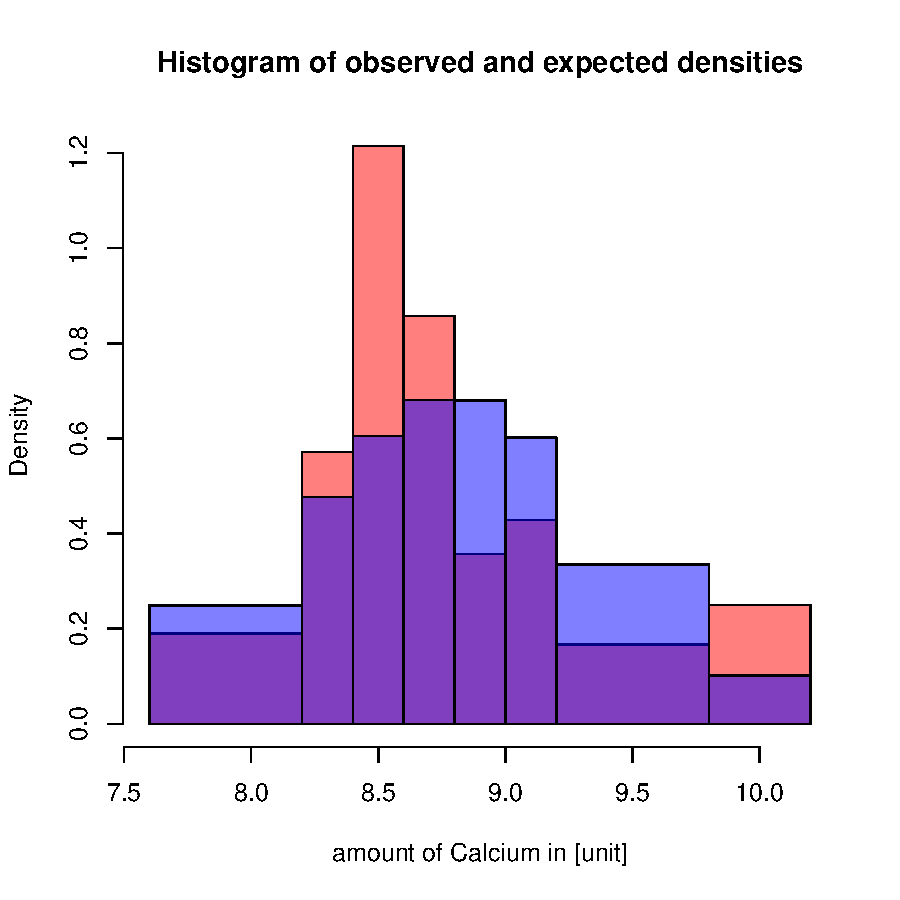
\includegraphics[width=0.8\textwidth]{report-chisqType1Ca}
\caption{Histogram of observed densities (red) and expected densities (blue) within the classes for the variable Calcium of type 1 glass}
\label{fig:chisqType1Ca}
\end{figure}

\begin{figure}[h!]
\centering
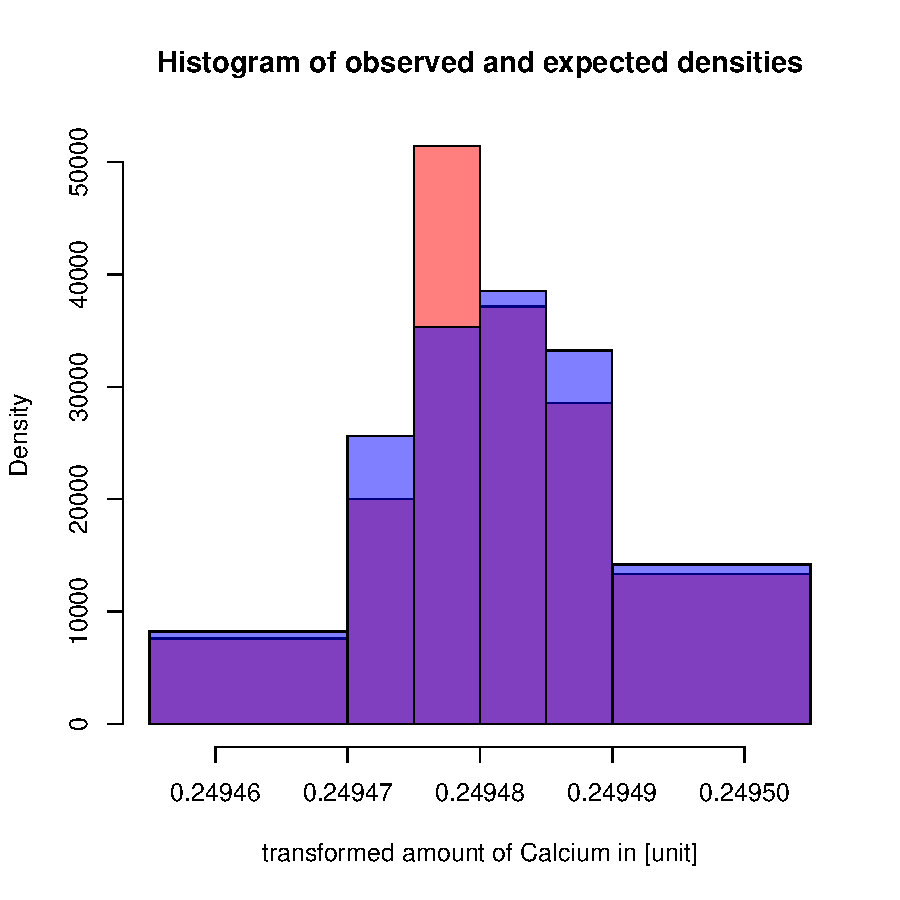
\includegraphics[width=0.8\textwidth]{report-chisqType1CaTrans}
\caption{Histogram of observed densities (red) and expected densities (blue) within the classes for transformed values of the variable Calcium of type 1 glass}
\label{fig:chisqType1CaTrans}
\end{figure}



Similar effects can be observed for the results of type 2 glass (table \ref{tab:chi-type2-trans}). Here, the hypothesis of normality is additionally not rejected for the variable Natrium.

\begin{table}[h!]
\centering
\begin{tabular}{|cccccc|} \hline variable & test statistic & sig. level & critical value & p-value & rejected\\ \hline RI & NA & 0.01 & NA & NA & NA\\ 
Na & 4.56 & 0.01 & 9.21 & 0.102375873496938 & no\\ 
Mg & NA & 0.01 & NA & NA & NA\\ 
Al & 2.61 & 0.01 & 13.28 & 0.62553471134666 & no\\ 
Si & 2.37 & 0.01 & 6.63 & 0.123314180710608 & no\\ 
K & NA & 0.01 & NA & NA & NA\\ 
Ca & 15.61 & 0.01 & 6.63 & 7.78625904057639e-05 & yes\\ 
Fe & NA & 0.01 & NA & NA & NA\\ \hline \end{tabular}\caption{Test results of the chi-squared test on the transformed data of type 2 glass with ten initial classes}
\label{tab:chi-type2-trans}
\end{table}

For the observations of type 7 glass, the test can now even be conducted on data of the variable Natrium, which were not properly distributed to perform the test before, \ie the data were not divided into a sufficient number of classes (table \ref{tab:chi-type7-trans}).

\begin{table}[h!]
\centering
\begin{tabular}{|cccccc|} \hline variable & test statistic & sig. level & critical value & p-value & rejected\\ \hline RI & NA & 0.01 & NA & NA & NA\\ 
Na & 1.83 & 0.01 & 6.63 & 0.176007215391275 & no\\ 
Al & 1.53 & 0.01 & 9.21 & 0.465771718543797 & no\\ 
Si & 12.46 & 0.01 & NA & NA & NA\\ 
K & NA & 0.01 & NA & NA & NA\\ 
Ca & 2.39 & 0.01 & NA & NA & NA\\ 
Ba & NA & 0.01 & NA & NA & NA\\ \hline \end{tabular}\caption{Test results of the chi-squared test on the transformed data of type 7 glass with ten initial classes}
\label{tab:chi-type7-trans}
\end{table}

\subsubsection{Kolmogorov-Smirnov test}

%<<calculatKSTrans, eval=TRUE, term=TRUE ,echo=FALSE>>=
%testresultKS.full.trans = apply(transformDataFrame(Glass[, -10]), 2, KSimpr.test.norm, sig=0.01)
%@
The first tests are conducted on the whole transformed data set for each
variable. No transformation data are given for RI, Mg, K, Ba, Fe - so no sense
for univariate transformation.

%The results are shown in table \ref{tab:KS-full}.

%\begin{table}[h!]
%\centering
%<<testresKSFullTrans, echo=FALSE, term=TRUE, results=tex>>=
%cat("\\begin{tabular}{|cccccc|} ")
%cat("\\hline ")
%cat(paste("variable & test statistic & sig. level & critical value & p-value & rejected\\\\ ", "\n", sep=""))
%cat("\\hline ")
%tr=testresultKS.full.trans
%
%for(i in 1:(length(tr))) {
%  cat(paste(
%    names(tr[i]),
%    round(tr[i][[1]]$teststat, 2),
%    0.01,
%    round(tr[i][[1]]$critical_value, 2),
%    ifelse(tr[i][[1]]$p_value < 1e-15, "< 1.0e-15", tr[i][[1]]$p_value),
%    ifelse(tr[i][[1]]$rejected, "yes", "no"),
%           sep=" & "), "\\\\ ", "\n", sep="")
%}
%
%cat("\\hline ")
%cat(paste("\\end{tabular}", "\n", sep=""))
%@
%\caption{Test results of the improved KS test on the whole transformed data
%sample with ten initial classes}
%\label{tab:KS-fullTrans}
%\end{table}


\newpage
\section{Conclusion}












\newpage
\section{Section 1}
Example for referring to a chapter: As written in section \ref{Intr} ...

  \subsection{First Subsection}
	Example for a citation: \cite{sqltuerker},\cite{journals/jods/VolzSM05}, \cite{das}\\
	%% you might need to compile the tex-file several times (pdfLaTeX, BibTeX, pdfLaTeX)
	%% in order to see the correct citations instead of question marks: "?"

	\begin{figure}[t!]
	\centering
	  
\includegraphics[height=0.49\textwidth,angle=90]{images/ercis.png}
	    \caption{Logo of ERCIS as an example for figures}
	  \label{ERCIS_Logo}
	\end{figure}

  \subsection{Second Subsection}

\newpage
\section{Section 2}
Here could be a table, e.g. table \ref{tab} (which is on page \pageref{tab}):

\begin{table}[ht] 
   \centering
      \begin{tabular}{|c||c|c|c|c|} \hline
			& \multicolumn{4}{c|}{Feature 2} 						\\
	Feature 1 & \multicolumn{2}{c|}{case} & \multicolumn{2}{c|}{studies}	\\
			& ca 			& te 		& go 	& ry 					\\ \hline \hline
	data 		& 63,50\% 	& 9,56\% 	& 2,16\% 	& 1,17\% 				\\ \hline
	analytics 	& 1,57\% 		& 0,41\% 	& 0,29\% 	& 0,41\% 				\\ \hline
      \end{tabular}
      \caption{This is the label of the table}
   \label{tab}
\end{table}


If you want to relate to a figure or table from a different page, you could do it this way: Figure \ref{ERCIS_Logo}, see page \pageref{ERCIS_Logo}, shows the ERCIS-Logo.

%%%%%%%%%%%%%%%%%%%%%%%%%%%%%%%%%%%%%%%%%%%%%%%%%%%%%%%%%%%%%%%%
%% appendix

\newpage

\begin{appendix}
\pagenumbering{roman}		%% roman page numbers for the appendix



\section{Appendix}

\begin{table}[h!]
\centering
\begin{tabular}{|cccccc|} \hline variable & test statistic & sig. level & critical value & p-value & rejected\\ \hline RI & 86.4 & 0.01 & 20.09 & 2.44249065417534e-15 & yes\\ 
Na & 49.04 & 0.01 & 23.21 & 3.99921126548186e-07 & yes\\ 
Mg & 668.81 & 0.01 & 16.81 & < 1.0e-15 & yes\\ 
Al & 61.72 & 0.01 & 29.14 & 5.84218540211623e-08 & yes\\ 
Si & 92.86 & 0.01 & 23.21 & 1.4432899320127e-15 & yes\\ 
K & 178.04 & 0.01 & 11.34 & < 1.0e-15 & yes\\ 
Ca & 149.63 & 0.01 & 18.48 & < 1.0e-15 & yes\\ 
Ba & 301.07 & 0.01 & 11.34 & < 1.0e-15 & yes\\ 
Fe & 137.37 & 0.01 & 18.48 & < 1.0e-15 & yes\\ \hline \end{tabular}\caption{Test results of the chi-squared test on the whole data sample with 30 initial classes}
\label{tab:chi-full-30}
\end{table}

\begin{table}[h!]
\centering
\begin{tabular}{|cccccc|} \hline variable & test statistic & sig. level & critical value & p-value & rejected\\ \hline RI & 102 & 0.01 & 13.28 & < 1.0e-15 & yes\\ 
Na & 16.61 & 0.01 & 18.48 & 0.0200763340092525 & no\\ 
Mg & 28.9 & 0.01 & 16.81 & 6.36733763034192e-05 & yes\\ 
Al & 27.56 & 0.01 & 16.81 & 0.000113486165164822 & yes\\ 
Si & 35.74 & 0.01 & 15.09 & 1.07201048937799e-06 & yes\\ 
K & 129.69 & 0.01 & 18.48 & < 1.0e-15 & yes\\ 
Ca & 20.22 & 0.01 & 18.48 & 0.00510775321781454 & yes\\ 
Fe & 45.28 & 0.01 & 9.21 & 1.46922363164492e-10 & yes\\ \hline \end{tabular}\caption{Test results of the chi-squared test on type 1 glass with 30 initial classes}
\label{tab:chi-type1-30}
\end{table}

\begin{table}[h!]
\centering
\begin{tabular}{|cccccc|} \hline variable & test statistic & sig. level & critical value & p-value & rejected\\ \hline RI & 77.84 & 0.01 & 15.09 & 2.33146835171283e-15 & yes\\ 
Na & 17.26 & 0.01 & 18.48 & 0.0157897896300554 & no\\ 
Mg & 306.84 & 0.01 & 15.09 & < 1.0e-15 & yes\\ 
Al & 20.77 & 0.01 & 20.09 & 0.00778471801730796 & yes\\ 
Si & 13.38 & 0.01 & 16.81 & 0.0374408380909446 & no\\ 
K & 54.24 & 0.01 & 13.28 & 4.67884619936854e-11 & yes\\ 
Ca & 106.11 & 0.01 & 11.34 & < 1.0e-15 & yes\\ 
Fe & 49.63 & 0.01 & 11.34 & 9.60126422810959e-11 & yes\\ \hline \end{tabular}\caption{Test results of the chi-squared test on type 2 glass with 30 initial classes}
\label{tab:chi-type2-30}
\end{table}

\begin{table}[h!]
\centering
\begin{tabular}{|cccccc|} \hline variable & test statistic & sig. level & critical value & p-value & rejected\\ \hline RI & 22.42 & 0.01 & 6.63 & 2.18961874765e-06 & yes\\ 
Na & 12.16 & 0.01 & 6.63 & 0.000489125271576851 & yes\\ 
Al & 3.37 & 0.01 & 9.21 & 0.185460070738202 & no\\ 
Si & 21.68 & 0.01 & 6.63 & 3.2242744996136e-06 & yes\\ 
K & 15.8 & 0.01 & NA & NA & NA\\ 
Ca & 11.55 & 0.01 & NA & NA & NA\\ 
Ba & 19.75 & 0.01 & 9.21 & 5.14515780526414e-05 & yes\\ \hline \end{tabular}\caption{Test results of the chi-squared test on type 7 glass with 30 initial classes}
\label{tab:chi-type7-30}
\end{table}

%%% to be deleted:
\begin{figure}[h!]
\centering
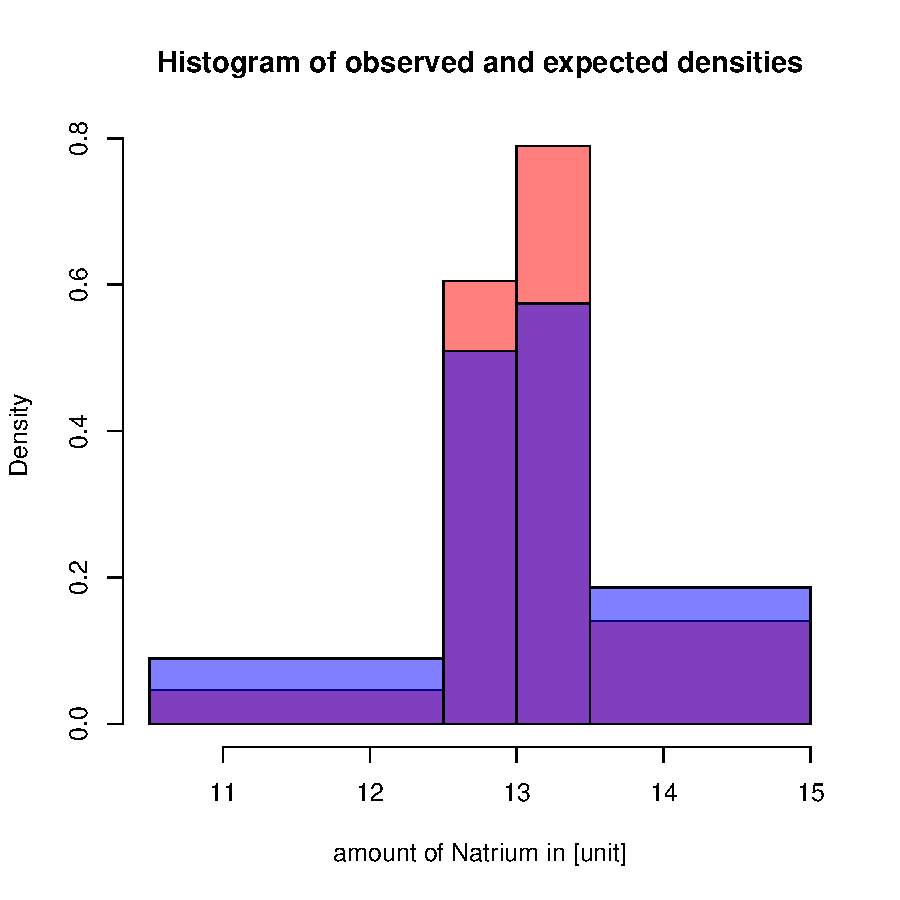
\includegraphics[width=0.6\textwidth]{report-chisqType2Na}
\caption{Histogram of observed densities (red) and expected densities (blue) within the classes for the variable Natrium of type 1 glass}
\label{fig:1}
\end{figure}

\begin{figure}[h!]
\centering
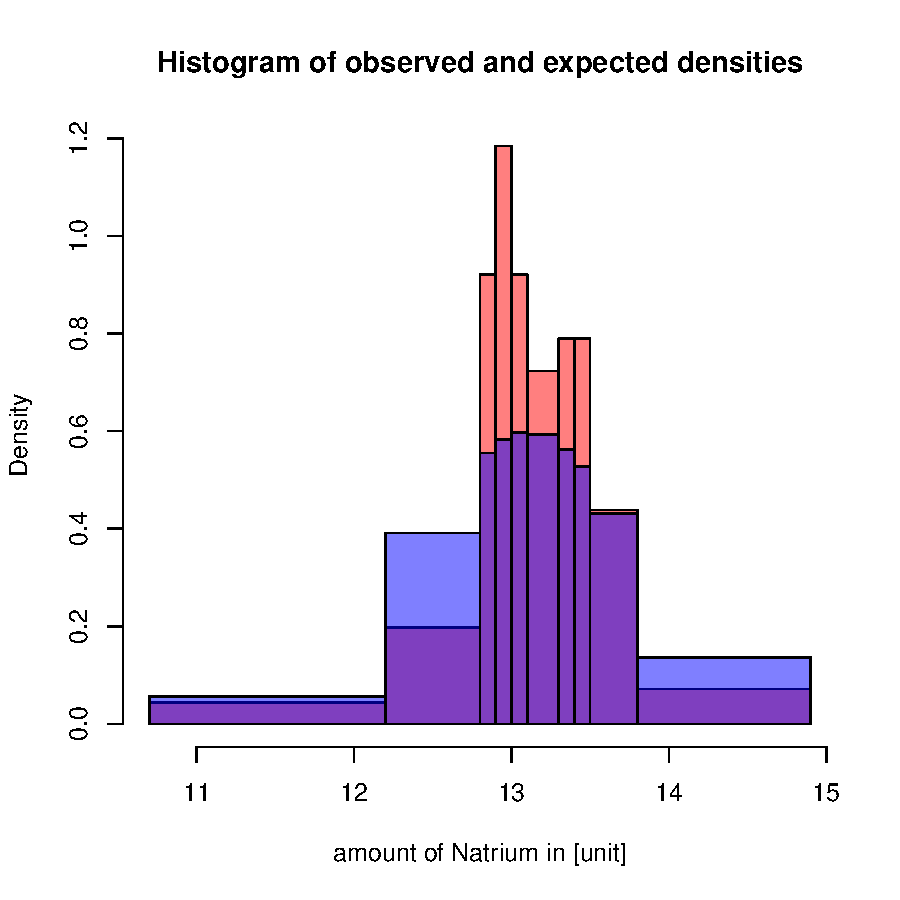
\includegraphics[width=0.6\textwidth]{report-chisqType2Na-30}
\caption{Histogram of observed densities (red) and expected densities (blue) within the classes for the variable Natrium of type 1 glass}
\label{fig:2}
\end{figure}

\begin{figure}[h!]
\centering
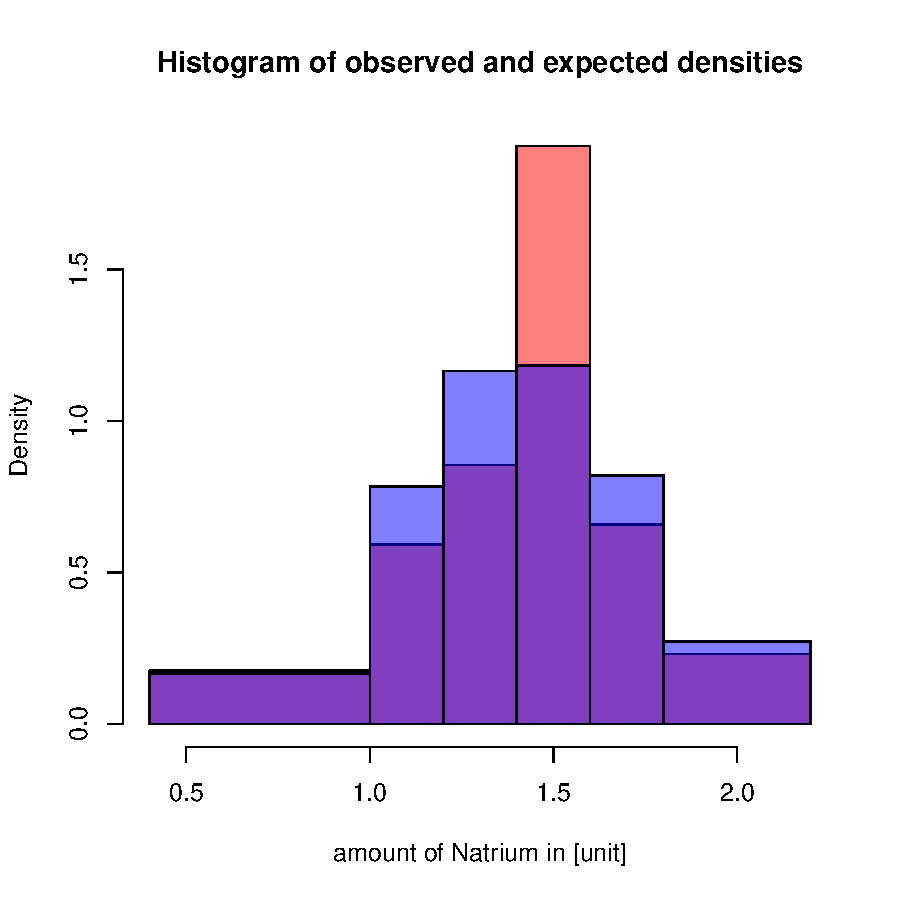
\includegraphics[width=0.6\textwidth]{report-chisqType2Al}
\caption{Histogram of observed densities (red) and expected densities (blue) within the classes for the variable Natrium of type 1 glass}
\label{fig:1}
\end{figure}

\begin{figure}[h!]
\centering
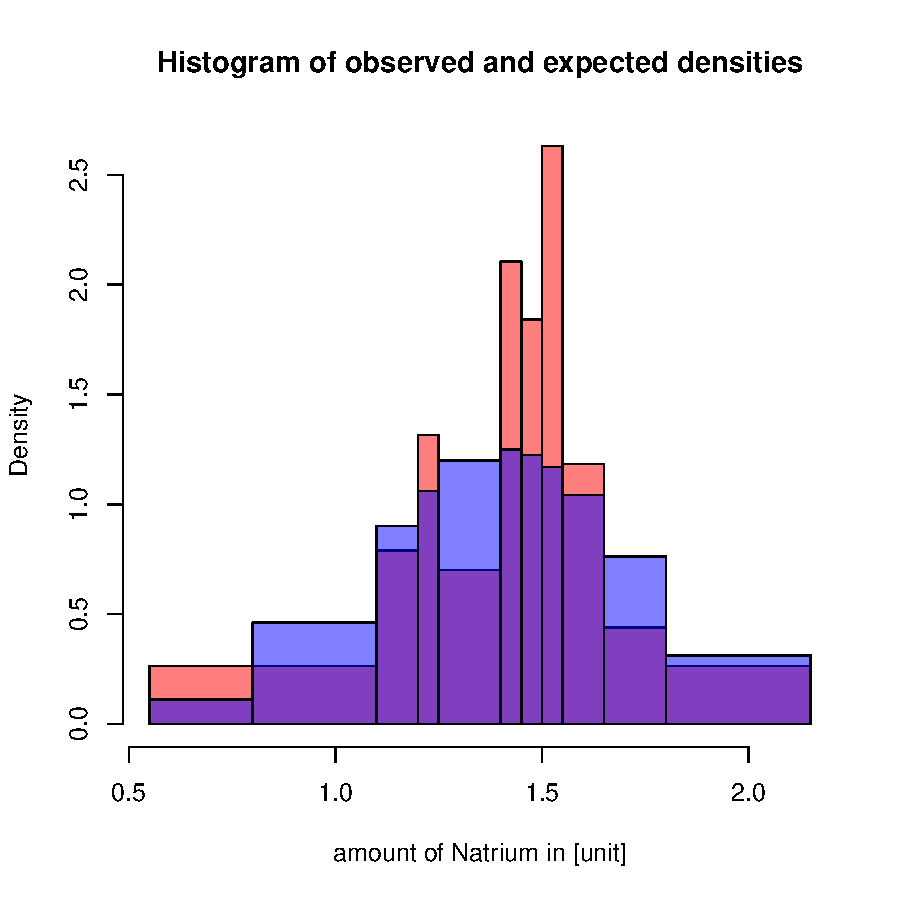
\includegraphics[width=0.6\textwidth]{report-chisqType2Al-30}
\caption{Histogram of observed densities (red) and expected densities (blue) within the classes for the variable Natrium of type 1 glass}
\label{fig:2}
\end{figure}

\end{appendix}

%%%%%%%%%%%%%%%%%%%%%%%%%%%%%%%%%%%%%%%%%%%%%%%%%%%%%%%%%%%%%%%%
%% lists of figures and tables

\newpage
\listoffigures
\listoftables

%%%%%%%%%%%%%%%%%%%%%%%%%%%%%%%%%%%%%%%%%%%%%%%%%%%%%%%%%%%%%%%%
%% bibliography (if needed)

%\nocite{*}
\bibliographystyle{plain}
\bibliography{lit}
%\bibitem[De02]{De02}DeGroot, Morris H., and Mark J. Schervish. Probability and
%Statistics.
% 3rd ed. Boston, MA: Addison-Wesley, 2002.
\end{document}
